% Template for PLoS
% Version 3.3 June 2016
%
% % % % % % % % % % % % % % % % % % % % % %
%
% -- IMPORTANT NOTE
%
% This template contains comments intended 
% to minimize problems and delays during our production 
% process. Please follow the template instructions
% whenever possible.
%
% % % % % % % % % % % % % % % % % % % % % % % 
%
% Once your paper is accepted for publication, 
% PLEASE REMOVE ALL TRACKED CHANGES in this file 
% and leave only the final text of your manuscript. 
% PLOS recommends the use of latexdiff to track changes during review, as this will help to maintain a clean tex file.
% Visit https://www.ctan.org/pkg/latexdiff?lang=en for info or contact us at latex@plos.org.
%
%
% There are no restrictions on package use within the LaTeX files except that 
% no packages listed in the template may be deleted.
%
% Please do not include colors or graphics in the text.
%
% The manuscript LaTeX source should be contained within a single file (do not use \input, \externaldocument, or similar commands).
%
% % % % % % % % % % % % % % % % % % % % % % %
%
% -- FIGURES AND TABLES
%
%  Please include tables/figure captions directly after the paragraph where they are first cited in the text.
%
%   DO NOT INCLUDE GRAPHICS IN YOUR MANUSCRIPT
% - Figures should be uploaded separately from your manuscript file. 
% - Figures generated using LaTeX should be extracted and removed from the PDF before submission. 
% - Figures containing multiple panels/subfigures must be combined into one image file before submission.
%   For figure citations, please use "Fig" instead of "Figure".
%   See http://journals.plos.org/plosone/s/figures for PLOS figure guidelines.
%
% Tables should be cell-based and may not contain:
% - spacing/line breaks within cells to alter layout or alignment
% - do not nest tabular environments (no tabular environments within tabular environments)
% - no graphics or colored text (cell background color/shading OK)
% See http://journals.plos.org/plosone/s/tables for table guidelines.
%
% For tables that exceed the width of the text column, use the adjustwidth environment as illustrated in the example table in text below.
%
% % % % % % % % % % % % % % % % % % % % % % % %
%
% -- EQUATIONS, MATH SYMBOLS, SUBSCRIPTS, AND SUPERSCRIPTS
%
% IMPORTANT
% Below are a few tips to help format your equations and other special characters according to our specifications. For more tips to help reduce the possibility of formatting errors during conversion, please see our LaTeX guidelines at http://journals.plos.org/plosone/s/latex
%
% For inline equations, please be sure to include all portions of an equation in the math environment.  For example, x$^2$ is incorrect; this should be formatted as $x^2$ (or $\mathrm{x}^2$ if the romanized font is desired).
%
% Do not include text that is not math in the math environment. For example, CO2 should be written as CO\textsubscript{2} instead of CO$_2$.
%
% Please add line breaks to long display equations when possible in order to fit size of the column. 
%
% For inline equations, please do not include punctuation (commas, etc) within the math environment unless this is part of the equation.
%
% When adding superscript or subscripts outside of brackets/braces, please group using {}.  For example, change "[U(D,E,\gamma)]^2" to "{[U(D,E,\gamma)]}^2". 
%
% Do not use \cal for caligraphic font.  Instead, use \mathcal{}
%
% % % % % % % % % % % % % % % % % % % % % % % % 
%
% Please contact latex@plos.org with any questions.
%
% % % % % % % % % % % % % % % % % % % % % % % %

\documentclass[10pt,letterpaper]{article}
\usepackage[top=0.85in,left=2in,footskip=0.75in]{geometry}

% amsmath and amssymb packages, useful for mathematical formulas and symbols
\usepackage{amsmath,amssymb}

% Use adjustwidth environment to exceed column width (see example table in text)
\usepackage{changepage}

% Use Unicode characters when possible
\usepackage[utf8x]{inputenc}

% textcomp package and marvosym package for additional characters
\usepackage{textcomp,marvosym}

% cite package, to clean up citations in the main text. Do not remove.
\usepackage{cite}

% Use nameref to cite supporting information files (see Supporting Information section for more info)
\usepackage{nameref,hyperref}

% line numbers
\usepackage[right]{lineno}

% ligatures disabled
\usepackage{microtype}
\DisableLigatures[f]{encoding = *, family = * }

% color can be used to apply background shading to table cells only
\usepackage[table]{xcolor}

% array package and thick rules for tables
\usepackage{array}

% create "+" rule type for thick vertical lines
\newcolumntype{+}{!{\vrule width 2pt}}

% create \thickcline for thick horizontal lines of variable length
\newlength\savedwidth
\newcommand\thickcline[1]{%
  \noalign{\global\savedwidth\arrayrulewidth\global\arrayrulewidth 2pt}%
  \cline{#1}%
  \noalign{\vskip\arrayrulewidth}%
  \noalign{\global\arrayrulewidth\savedwidth}%
}

% \thickhline command for thick horizontal lines that span the table
\newcommand\thickhline{\noalign{\global\savedwidth\arrayrulewidth\global\arrayrulewidth 2pt}%
\hline
\noalign{\global\arrayrulewidth\savedwidth}}


% Remove comment for double spacing
%\usepackage{setspace} 
%\doublespacing

% Text layout
\raggedright
\setlength{\parindent}{0.5cm}
\textwidth 5.25in 
\textheight 8.75in

% Bold the 'Figure #' in the caption and separate it from the title/caption with a period
% Captions will be left justified
\usepackage[aboveskip=1pt,labelfont=bf,labelsep=period,justification=raggedright,singlelinecheck=off]{caption}
\renewcommand{\figurename}{Fig}

% Use the PLoS provided BiBTeX style
\bibliographystyle{plos2015}

% Remove brackets from numbering in List of References
\makeatletter
\renewcommand{\@biblabel}[1]{\quad#1.}
\makeatother

% Leave date blank
\date{}

% Header and Footer with logo
\usepackage{lastpage,fancyhdr,graphicx}
\usepackage{epstopdf}
\pagestyle{myheadings}
\pagestyle{fancy}
\fancyhf{}
\setlength{\headheight}{27.023pt}
\lhead{
\includegraphics[width=3.0in]{PLOS-submission.eps}}
\rfoot{\thepage/\pageref{LastPage}}
\renewcommand{\footrule}{\hrule height 2pt \vspace{2mm}}
\fancyheadoffset[L]{1.25in}
\fancyfootoffset[L]{1.25in}
\lfoot{\sf PLOS}

%% Include all macros below

\newcommand{\lorem}{{\bf LOREM}}
\newcommand{\ipsum}{{\bf IPSUM}}

%% END MACROS SECTION

\begin{document}
\vspace*{0.2in}

% Title must be 250 characters or less.
\begin{flushleft}
{\Large
\textbf\newline{Research Synergy and Drug Development: Bright Stars in Neighboring Constellations} % Please use "title case" (capitalize all terms in the title except conjunctions, prepositions, and articles).
}
\newline
% Insert author names, affiliations and corresponding author email (do not include titles, positions, or degrees).
\\
Samet Keserci\textsuperscript{1},
%Samet Keserci\textsuperscript{1,2\Yinyang},
Eric Livingston\textsuperscript{2},
Lingtian Wan\textsuperscript{1,\textcurrency},
Alexander R. Pico\textsuperscript{3},
%Name5 Surname\textsuperscript{2\ddag},
%Name6 Surname\textsuperscript{2\ddag},
 \& George Chacko\textsuperscript{1*}
%with the Lorem Ipsum Consortium\textsuperscript{\textpilcrow}
\\
\bigskip
\textbf{1} Netelabs, NET ESolutions Corporation, McLean, VA, USA
\\
\textbf{2} Elsevier Research Intelligence, Elsevier Inc., Bethesda, MD, USA
\\
\textbf{3} Gladstone Institutes, University of California San Francisco, San Francisco, CA, USA
\\
\bigskip

% Insert additional author notes using the symbols described below. Insert symbol callouts after author names as necessary.
% 
% Remove or comment out the author notes below if they aren't used.
%
% Primary Equal Contribution Note
%\Yinyang These authors contributed equally to this work.

% Additional Equal Contribution Note
% Also use this double-dagger symbol for special authorship notes, such as senior authorship.
%\ddag These authors also contributed equally to this work.

% Current address notes
\textcurrency Current Address: Facebook Corporation, Menlo Park, CA, USA % change symbol to "\textcurrency a" if more than one current address note
% \textcurrency b Insert second current address 
% \textcurrency c Insert third current address

% Deceased author note
%\dag Deceased

% Group/Consortium Author Note
%\textpilcrow Membership list can be found in the Acknowledgments section.

% Use the asterisk to denote corresponding authorship and provide email address in note below.
*Correspondence: george@nete.com
\end{flushleft}
% Please keep the abstract below 300 words
\section*{Abstract}

Drug discovery and the subsequent availability of new breakthrough therapeutics or `cures' are compelling examples of societal benefit from advances in research. Such advances are invariably collaborative, involving the contributions of many scientists in a `cure network' where prior theory and experiment is built upon. Data mining of public and commercial data sources coupled with network analysis is a scalable digital methodology for assembling and analyzing the history of scientific advances. This methodology is extensible beyond cure networks and its use supports (i) efficiency in  exploring  the scientific history of a research advance (ii) improved documenting and understanding of collaboration (iii) portfolio analysis, planning and optimization (iv) communication of the societal value of research. Building upon prior techniques for single cure networks and linking the work of approximately 200,000 authors in 100,000 scientific publications, we have conducted a case study of five anti-cancer therapeutics for the purpose of exploring the relationship across networks. We have enriched the content of these five networks by annotating them with information on research awards as well as peer review that preceded these awards. Applying retrospective citation discovery, we have identified a core set of publications cited in the networks of all five therapeutics and additional intersections in combinations of networks as well as a core set of awards from the National Institutes of Health that supported this research. Lastly, we have mapped these awards to their cognate peer review panels, identifying another layer of collaborative scientific activity that influenced the research represented by these networks. 

% Please keep the Author Summary between 150 and 200 words
% Use first person. PLOS ONE authors please skip this step. 
% Author Summary not valid for PLOS ONE submissions.   
%\section*{Author Summary}
%Lorem ipsum dolor sit amet, consectetur adipiscing elit. Curabitur eget porta erat. Morbi consectetur est vel gravida pretium. Suspendisse ut dui eu ante cursus gravida non sed sem. Nullam sapien tellus, commodo id velit id, eleifend volutpat quam. Phasellus mauris velit, dapibus finibus elementum vel, pulvinar non tellus. Nunc pellentesque pretium diam, quis maximus dolor faucibus id. Nunc convallis sodales ante, ut ullamcorper est egestas vitae. Nam sit amet enim ultrices, ultrices elit pulvinar, volutpat risus.

\linenumbers
% Use "Eq" instead of "Equation" for equation citations.
\section*{Introduction}

Data mining of public data sources coupled with network analysis allows the assembly and quantitative description of research discoveries that were influential in the development of a breakthrough therapeutic or `cure'.  The set of scientific publications, clinical trials, patents, and regulatory approvals, linked to each other by citation or assignment, that documents progress from basic research to a cure is termed a `cure network' \cite {bib1}. Key assumptions in constructing these networks are that the references found in relevant documents are appropriate citations of new knowledge relevant to a given cure and that a further retrospective round of citation discovery will uncover previous influential discovery (\textit{ibid}). Williams and colleagues have elegantly demonstrated the feasibility of this approach using, as case studies, ivacaftor and ipilimumab, approved for the treatment of cystic fibrosis and melanoma respectively (\textit{vide supra}). These authors observed that `the nature of a cure discovery network is complex and fundamentally collaborative', noting in the case of ivacaftor, that at least 7,067 scientists with 5,666 unique affiliations contributed to ivacaftor-related research over a period greater than 100 years. 

Such studies provide evidence for the broad collaborative platform of basic and translational research underlying major scientific advances such as cures for diseases, support strategic communications to oversight bodies, and communication of the societal value of research\cite {bib2,bib3}. Extending this digital methodology to study additional cures as well as significant research advances in general is a logical next step. Ascertaining the nature of the interactions, if any, between networks, is also of considerable interest since it would support an understanding of collaboration across networks as well as common features of science networks.  

To address these questions, we have conducted case studies of a cluster of five FDA-approved therapeutics for cancer. We have extended the original approach to (i) include a data from a commercially available bibliographic database with disambiguated author identifiers (ii) modified the original data mining methods and network metrics (iii) added new node types to include grants and peer review data (iv) refactored the network analysis code of Williams et al. for better performance. (v) mapped publications and authors across all five networks. 

We present the results of these case studies as a step towards mapping the universe of FDA-approved drugs and biologicals. Beyond drug discovery and cures, however, this simple digital methodology can be used to support efficient explorations of science history, gain an understanding of collaboration across domains, enrich portfolio analysis, planning and optimization, enable communications of the societal value of research, and help make the scientific environment more citizen-accessible. 

\section*{Materials and Methods} 
% Place tables after the first paragraph in which they are cited.
A set of five anti-cancer therapeutics, three drugs and two biologicals, approved for use in humans by the Food and Drug Administration was selected for this study (Table 1). Imatinib and Sunitinib are tyrosine kinase inhibitors, Nelarabine is a nucleoside analog, and Ramucirumab and Alemtuzumab are humanized antibodies that target cell surface receptors. 
 For each of these therapeutics, a set of relevant scientific publications was constructed as in Williams et al.\cite{bib1} but with specific modifications detailed below. An allowance of 2 months was made for `publication lag' when assembling referenced material. For example, if a therapeutic was approved on Jan 1, 2017, documents published  on or before March 31, 2017 were included. For each of the five therapeutics, a first-generation list of PubMed identifiers (citing\_pmid) was harvested from the five different data sources (below).  
\begin{table}[!ht]
%\begin{adjustwidth}{-0.5in}{0in} % Comment out/remove adjustwidth environment if table fits in text column.
\centering
\scalebox{0.9}{
\begin{tabular}{|l+l|l|l|l|l|l|l|}
\hline
%\multicolumn{4}{|l|}{\bf Heading1} & \multicolumn{4}{|l|}{\bf Heading2}\\ \thickhline
Therapeutic & FDA Approval Date & Unique Identifier & US Patent & Publication Date  \\ \hline
$Alemtuzumab$ & May 2001 & BLA: 103948 & US5846534 & Dec 1998\\ \hline
$Imatinib$ & May 2001 & NDA: 021335 & US5521184 &  May 1996 \\ \hline
$Nelarabine$ & Oct 2005 & NDA: 021877 & US5424295 & Jun 1995  \\ \hline
$Ramucirumab$ & Apr 2014 & BLA: 125477 & US7498414 & Mar 2009  \\ \hline
$Sunitinib$ & Jan 2006  & NDA: 021938  & US6573293 & Jun 2003 \\ \hline
\end{tabular}}
\vspace{2 mm}
\caption{
{\bf Case Studies of Five Anti-Cancer Agents} Five anti-cancer therapeutics, with FDA approval dates ranging from 2001 to 2014, were selected as case studies. The active ingredient for each of these five therapeutics is listed in column 1. While multiple patents are typically associated with a drug or biological, the single US patent number displayed represents the primary invention that preceded approval of the therapeutic. The publication date for each patent is listed in the last column.}
%\begin{flushleft}  
%\end{flushleft}
\label{table1}
%\end{adjustwidth}
\end{table}

\textbf{Clinical trials} The national clinical trials database (clinicaltrials.gov) was searched for clinical trials of the five therapeutics that completed on or the data of FDA approval. Both cited references and publications from these clinical trials were collected if they were published within the approval date plus two months. To capture publications associated with the clinical trials that were not displayed in clinical trials.gov, PubMed was also searched with the unique identifier (NCT number) of any clinical trials that were identified. To capture publications of clinical trials not registered in clinicaltrials.gov, PubMed was searched using the therapeutic name as keyword, publication type as ``clinical trial'', and an appropriate date restriction as in searches of clinicaltrials.gov. For example, the search term (((``alemtuzumab"[Supplementary Concept] OR ``alemtuzumab"[All Fields]) OR (``alemtuzumab"[Supplementary Concept] OR ``alemtuzumab"[All Fields] OR ``campath"[All Fields])) AND (``1900/0101"[PDAT] : ``2001/07/31''[PDAT])) AND ``clinical trial"[Publication Type] was used to identify publications of clinical trials for Alemtuzumab.

\textbf{FDA documents} The drugs@fda website\cite{bib6} was searched for each of the five therapeutics and cited references in the medical review document were manually extracted and matched to pmids. FDA Approval Summaries, articles published in journals by FDA staff, were available for all five therapeutics and contain cited references. If the published date of a citation exceeded the approval date plus two months, the publication was not included.

\textbf{Patents} For each therapeutic a single patent was identified that best represented the most relevant invention to the therapeutic at hand. Identification of this patent was performed using multiple web sources. The US patent number was then used to identify the patent and the non-patent citation list from Google Patents \cite{bib8} was manually processed by searching PubMed for appropriate pmids. While we developed a citation matching tool for non-patent literature for this purpose, the accuracy of manual searches was far higher and were used to generate the data in this study.

\textbf{Post-approval literature reviews} Review articles published after a therapeutic's approval by the FDA are independent assessments of the the development of a therapeutic. Accordingly, PubMed was searched for review articles of a therapeutic that were published between the date of FDA approval and one year following the date of approval and cited references in these reviews were extracted using PubMed and Scopus.

\textbf{Pre-approval literature searches} Literature searches were performed using PubMed with a date range of 1900/01/01 to two months post-FDA approval. For example, the search term ((alemtuzumab) OR campath) AND (``1900/01/01"[Date - Publication] : ``2001/07/31"[Date - Publication]) was used to retrieve articles of interest relevant to alemtuzumab.

Citing\_pmids from the five different sources above  were combined and deduplicated. Using the Scopus database and its APIs, these citing\_pmids were mapped to Scopus identifiers (citing\_sid) from which a second generation of cited references (cited\_sid) was extracted., These cited\_sids, were in turn, mapped back to pmids (cited\_pmid). Whereas mapping between PubMed and Scopus identifiers at the citing\_pmid and citing\_sid stage resulted in 1\% or less information loss, mapping at the cited\_sid to cited\_pmid resulted in 15-20 \% information loss. Accordingly the Scopus data  was used as the backbone of the publication component of the network and the cited\_pmid information was treated as an annotation layer.  These observations are summarized in Table 2 and include the count of null values when mapping from citing\_sid to cited\_sid.

Citing and cited pmids were both mapped to NIH grants and peer review panels using information made publicly available by NIH through NIH ExPORTER. Since Special Emphasis Panels vary in scientific interests from year to year, we restricted our mapping to chartered study sections, which have defined scientific interests and relatively stable reviewer membership. The resultant data were modeled as hierarchical networks and analyzed using metrics based on network topology. We calculated the propagated in-degree rank (PIR) metric of Williams \cite {bib1}. PIR represents the sum of weighted citation scores for all articles in a network that can be attributed to an author. In addition to computing PIR for all authors in each network, we also combined the citation data for all five networks and computed a globalPIR score, which was normalized to the sum of PIR scores within each network.

We also calculated the RBR metric of Williams et al. (\textit{ibid}) with some modifications. The RBR metric is intended to represent the fraction of a researcher's output that is in a network and is defined as the ratio of the number of publications in network to the number of publications in a background dataset for an author. In its original specification, the background dataset for RBR was constructed by keyword searches of PubMed. A potential weakness of this keyword based approach is that keywords do not effectively capture the field or the total output of an author even if multiple background samples are taken. Therefore, we created two new variants of the RBR; network RBR (nRBR) and document-based RBR (dRBR). nRBR uses all publications in our set of five therapeutics as background and dRBR takes advantage of the Scopus author\_id to capture the total output of an author and use it as background. Thus, nRBR and dRBR normalize a researcher's in-network contributions to backgrounds based on total network and total researcher productivity respectively.\\
\vspace{2.5 mm}


\textbf{Notation and Calculations}
\begin {itemize}
\item $d_i =$  therapeutic, e.g., alemtuzumab(alem) or imatinib(imat)
\item $N_i =$ the network of a therapeutic $d_i$;
\item $\mathcal{N}$ = union of all networks $N_i$
\item $\mathcal{G}$ the global network - the set of all authors and publications in $\mathcal{N}$ 
\item $\mathcal{M}$ the set of all subnetworks - ie $\{N_1,N_2,N_3,N_4,N_5\}$
\item $c_n(\mathfrak{p})$ citation of a publication $\mathfrak{p}$ in a network $n$
\item $\mathcal{C}_\mathfrak{p}^n$ =the set of publications which cites $\mathfrak{p}$ in a network $n$
\item $wc_n(\mathfrak{p})$  weighted citation of a publication $\mathfrak{p}$ in a network $n$
\item $\mathcal{A}_\mathfrak{a}^n$ the set of publications for an author $\mathfrak{a}$ in a network $n$
\item $pir_n(\mathfrak{a})$ the PIR  score of an author in a Network $n$ in $\mathcal{M}$
\item $npir(\mathfrak{a})$ the PIR score of an author  $\mathfrak{a}$ in the Network  $\mathcal{N}$ 
\item $ir(\mathfrak{a})$ partitioning of a research metric for an author $\mathfrak{a}$ 
\item $ic_{d_i}(\mathfrak{a})$ = total \# in-degree count for an author $\mathfrak{a}$  for drug $d_i$. (ie. = $\|\mathcal{A}_\mathfrak{a}^{d_i}\|$)
\item $ic_n(\mathfrak{a})$ = total \# in-degree count for an author $\mathfrak{a}$  in  $\mathcal{N}$ (i.e = $\|\mathcal{A}_\mathfrak{a}^{N}\|$)
\item $ nrbr_{d_i}(\mathfrak{a}) $ modified RBR score normalized to its network $\mathcal{N}$ for a drug $d_i$
\item $ grbr_{d_i}(\mathfrak{a}) $ modified RBR score normalized to the global network $\mathcal{G}$  for a drug $d_i$
\end{itemize}

\textbf{PIR Score}: We define the global network $\mathcal{N}$ as the union of the each individual sub-network of a therapeutic $d_i$. In other words 
$$ \mathcal{N} = \cup_{i =1}^{5} \mathcal{N}_i $$
Let $c_n(\mathfrak{p})$ be the citation score of the the paper $\mathfrak{p}$ in a network $n$, and $\mathcal{C}_\mathfrak{p}^n$ be the set of publication which cites $\mathfrak{p}$. Then we define the weighted citation of a paper $\mathfrak{p}$ as $$wc_n(\mathfrak{p}) = c_n(\mathfrak{p}) + \sum_{g\in \mathcal{C}_\mathfrak{p}^n}  c_n(g) $$
Let $\mathcal{A}_a^n$ be the set of publications for an author $\mathfrak{a}$ in a Network $n$. Then the PIR score  for an author $\mathfrak{a}$  in network $n$ is defined as $$ pir_n(\mathfrak{a}) =  \sum_{p\in \mathcal{A}_a^n}  wc_n(\mathfrak{p}) $$

More simply, the PIR score for an author  $\mathfrak{a}$ in a Network $n$ is  $$ pir_n(\mathfrak{a}) =  \sum_{p\in \mathcal{A}_a^n } \big[c_n(p) + \sum_{g\in \mathcal{C}_\mathfrak{p}^n}  c_n(g)\big] $$

Next we define the nPIR score $npir(\mathfrak{a})$, which is $pir$ score based on the  total network $\mathcal{N}$. For convenience, instead of denoting it $pir_N$, we use $npir$   Furthermore  we define the isolation of  research  metric $ir(\mathfrak{a}):\mathcal{R}\rightarrow [1,\infty]$  of an author $\mathfrak{a}$ as 
$$ir(\mathfrak{a})= \dfrac{ npir({\mathfrak{a}})} {\sum_{1}^{5} pir_{d_i}(\mathfrak{a})} $$
where $\mathcal{R}$ is the set of all authors in $\mathcal{N}$  and  $pir_{d_i}(\mathfrak{a})$ is the PIR score of the author $\mathfrak{a}$ restricted to only drug network $\mathcal{D}_i$ . If $ir(\mathfrak{a})$ approaches 1, the author's $\mathfrak{a}$ contribution to each drug is partitioned. The greater the $ir$, the closer  the interaction of the author's papers between the networks. 

\textbf{RBR Score}:
\begin{itemize}
\item nRBR or network RBR is the ratio of an authors' count of publications in a network to the total number of the publications in the global Network. 
Lets define in-degree count $ic_{d_i}(\mathfrak{a})$ of an author $\mathfrak{a}$ as the total number of the publication which is in the network $\mathcal{N}_i$ of the drug $d_i$, similarly lets $ic_{n}$ be the number of the paper that author $\mathfrak{a}$ published in the total Network(5-drug's network) $\mathcal{N}$. Then we define, nRBR of an author $\mathfrak{a}$  for a drug $d_i$ as follow.
$$ nrbr_{d_i}(\mathfrak{a}) = \dfrac{ic_{d_i}(\mathfrak{a})}{ic_{N}(\mathfrak{a})}$$
\item gRBR or global RBR is the ratio of an author's count of publications in a network to the author's total publication count. $\mathcal{G}$. Thus, $grbr$ score of an author  $\mathfrak{a}$  for the drug $d_i$ is defined as 
$$grbr_{d_i}(\mathfrak{a}) = \dfrac{ic_{d_i}(\mathfrak{a})}{ic_{G}(\mathfrak{a})}$$
where $ic_{G}$ is the total number of publication that an author $\mathfrak{a}$ currently has.
\end{itemize}

\subsection*{Etiam eget sapien nibh.}

% For figure citations, please use "Fig" instead of "Figure".
Nulla mi mi, Fig~\ref{fig1} venenatis sed ipsum varius, volutpat euismod diam. Proin rutrum vel massa non gravida. Quisque tempor sem et dignissim rutrum. Lorem ipsum dolor sit amet, consectetur adipiscing elit. Morbi at justo vitae nulla elementum commodo eu id massa. In vitae diam ac augue semper tincidunt eu ut eros. Fusce fringilla erat porttitor lectus cursus, \nameref{S1_Video} vel sagittis arcu lobortis. Aliquam in enim semper, aliquam massa id, cursus neque. Praesent faucibus semper libero.

% Place figure captions after the first paragraph in which they are cited.


% Results and Discussion can be combined.
\section*{Results and Discussion}

Scientific publications form the backbone of each of these five networks. The initial assumptions of appropriate citation and retrospective citation discovery (Introduction) suggest that network nodes that are common to multiple networks are likely to be influential. Accordingly. we explored the extent and nature of intersections across networks, we calculated intersection counts for all possible combinations of Alemtuzumab, Imatinib, Nelarabine, Ramucirumab, and Sunitinib (Table 3). 14 publications are cited in all five networks and are shown in Table 4. 

\begin{table}[!ht]
\begin{adjustwidth}{-1.0in}{0in} % Comment out/remove adjustwidth environment if table fits in text column.
\centering
\scalebox{0.8}{\begin{tabular}{|l+l|l|l|l|l|l|l|}
\hline
%\multicolumn{4}{|l|}{\bf Heading1} & \multicolumn{4}{|l|}{\bf Heading2}\\ \thickhline
\hline
SourceYear & SourceName & Author(s) \\ 
  \hline
1958 & J. Am. Stat. Assoc. & Kaplan E.R., Meier P. \\ 
1963 & Science & Jerne, N. K. and Nordin, A. A.  \\ 
1972 & J R Stat Soc & Cox DR.  \\ 
1976 & Anal. Biochem. & Bradford MM \\ 
1977 & Br J Cancer & R. Peto, M.C. Pike, and P. Armitage  \\ 
1977 & Proc. Natl. Acad. Sci. & Sanger, F., S. Nicklen, and A.R. Coulson.  \\ 
1983 & J Immunol Methods & Mosmann T  \\ 
1984 & Adv Enzyme Regul & T.C. Chou, and P. Talalay  \\ 
1989 & Molecular Cloning: A Laboratory Manual & Sambrook, J., Fritsch, E. and Maniatis, T.  \\ 
1994 & Acta Crystallogr D & Collaborative Computational Project 4 \\ 
1994 & Acta Crystallogr. A & Navaza J.  \\ 
1997 & Cell & Levine, A. J. \\ 
1997 & Am. J. Pathol. & Perez-Atayde, A. R., Sallan, S. E., Tedrow, U., Connors, S., Allred, E., and Folkman, J.  \\ 
1998 & CA: A Cancer Journal for Clinicians & SH Landis T Murray S Bolden PA Wingo \\ 
\hline
\end{tabular}}
\vspace{2.5 mm}
\caption{{\bf Citation Counts and Mapping Between Bibliographic Databases} Five anti-cancer therapeutics were selected as case studies. A foundational set of references (citing\_pmid) was assembled for each therapeutic from patents, clinical trials, regulatory documents, and the scientific literature. Citing\_pmids were mapped to Scopus identifiers (citing\_sid), which were used, in turn, to retrieve literature cited by this foundational set (cited\_sid). Cited\_sids were mapped back to PubMed identifiers (cited\_pmid).The number of  identifiers at each stage of the mapping process is shown along with percentage loss (in parentheses) when mapping across PubMed and Scopus or due to null values in the cited\_sid field} 
\label{table4}
\end{adjustwidth}
\end{table}

Thus, we also applied intersection analysis as above at a finer level of granularity by computing intersection counts for first generation citations (citing\_pmid) and second generation citations (cited\_sid). The results are displayed as Venn diagrams in Figures 1 and 2 respectively. Strikingly, no publications are common to all five networks at the first generation level although a single publication, the highly influential work of Kohler and Milstein\cite{bibKohler}, is cited in four out of five networks. All 14 publications cited in our set of five networks were in the second generation of citations and another 198 were found  across various the four-network combinations, roughly an order of magnitude greater than the case of cited references.  We manually grouped the 14 publications using high level descriptive terms and noted statistical techniques (5 publications), molecular and cell biological methods (4), analytical and structural biochemistry techniques (3) and cancer biology (2). Of these last two, one is a review of the p53 gene [cite] and the second is a study of angiogenesis in children with acute lymphoblastic leukemia [cite]. Thus, the majority of this small set of 14 publications concerns methods that are heavily cited in these therapeutic development networks. We are actively working on characterizing the entire dataset as well as intersecting subsets using methods that would scale to thousands of publications and these results will be shared in another publication [needs to be reworded].

\begin{table}[!ht]
%\begin{adjustwidth}{-0.5in}{0in} % Comment out/remove adjustwidth environment if table fits in text column.
\centering
\scalebox{0.9}{
\begin{tabular}{|l+l|l|l|l|l|l|l|}
\hline
%\multicolumn{4}{|l|}{\bf Heading1} & \multicolumn{4}{|l|}{\bf Heading2}\\ \thickhline
Therapeutic & citing\_pmid count & citing\_sid count & cited\_sid count  & cited\_pmid count  \\ \hline
$Alemtuzumab$ & 599 & 587 (1\%) & 8840 (2\%) & 7071(20\%)\\ \hline
$Imatinib$ & 1380 & 1373(1\%) & 27326(1\%) &  23340(17\%) \\ \hline
$Nelarabine$ & 104 & 104(0\%) & 2476(1\%) & 1990(20\%)  \\ \hline
$Ramucirumab$ & 1820 & 1804(1\%) & 48587(0\%) & 40973(19\%)  \\ \hline
$Sunitinib$ & 1512  & 1509(0\%)  & 33895(0\%) & 28661(15\%) \\ \hline
\end{tabular}
}
\vspace{2.5 mm}
\caption{{\bf Citation Counts and Mapping Between Bibliographic Databases} Five anti-cancer therapeutics were selected as case studies. A foundational set of references (citing\_pmid) was assembled for each therapeutic from patents, clinical trials, regulatory documents, and the scientific literature. Citing\_pmids were mapped to Scopus identifiers (citing\_sid), which were used, in turn, to retrieve cited publications (cited\_sid). Cited\_sids were mapped back to PubMed identifiers (cited\_pmid).The number of  identifiers at each stage of the mapping process is shown along with percentage loss (in parentheses) when mapping across PubMed and Scopus or due to null values in the cited\_sid field} 
\label{table2}
%\end{adjustwidth}
\end{table}


\begin{figure}[!h]
\centering
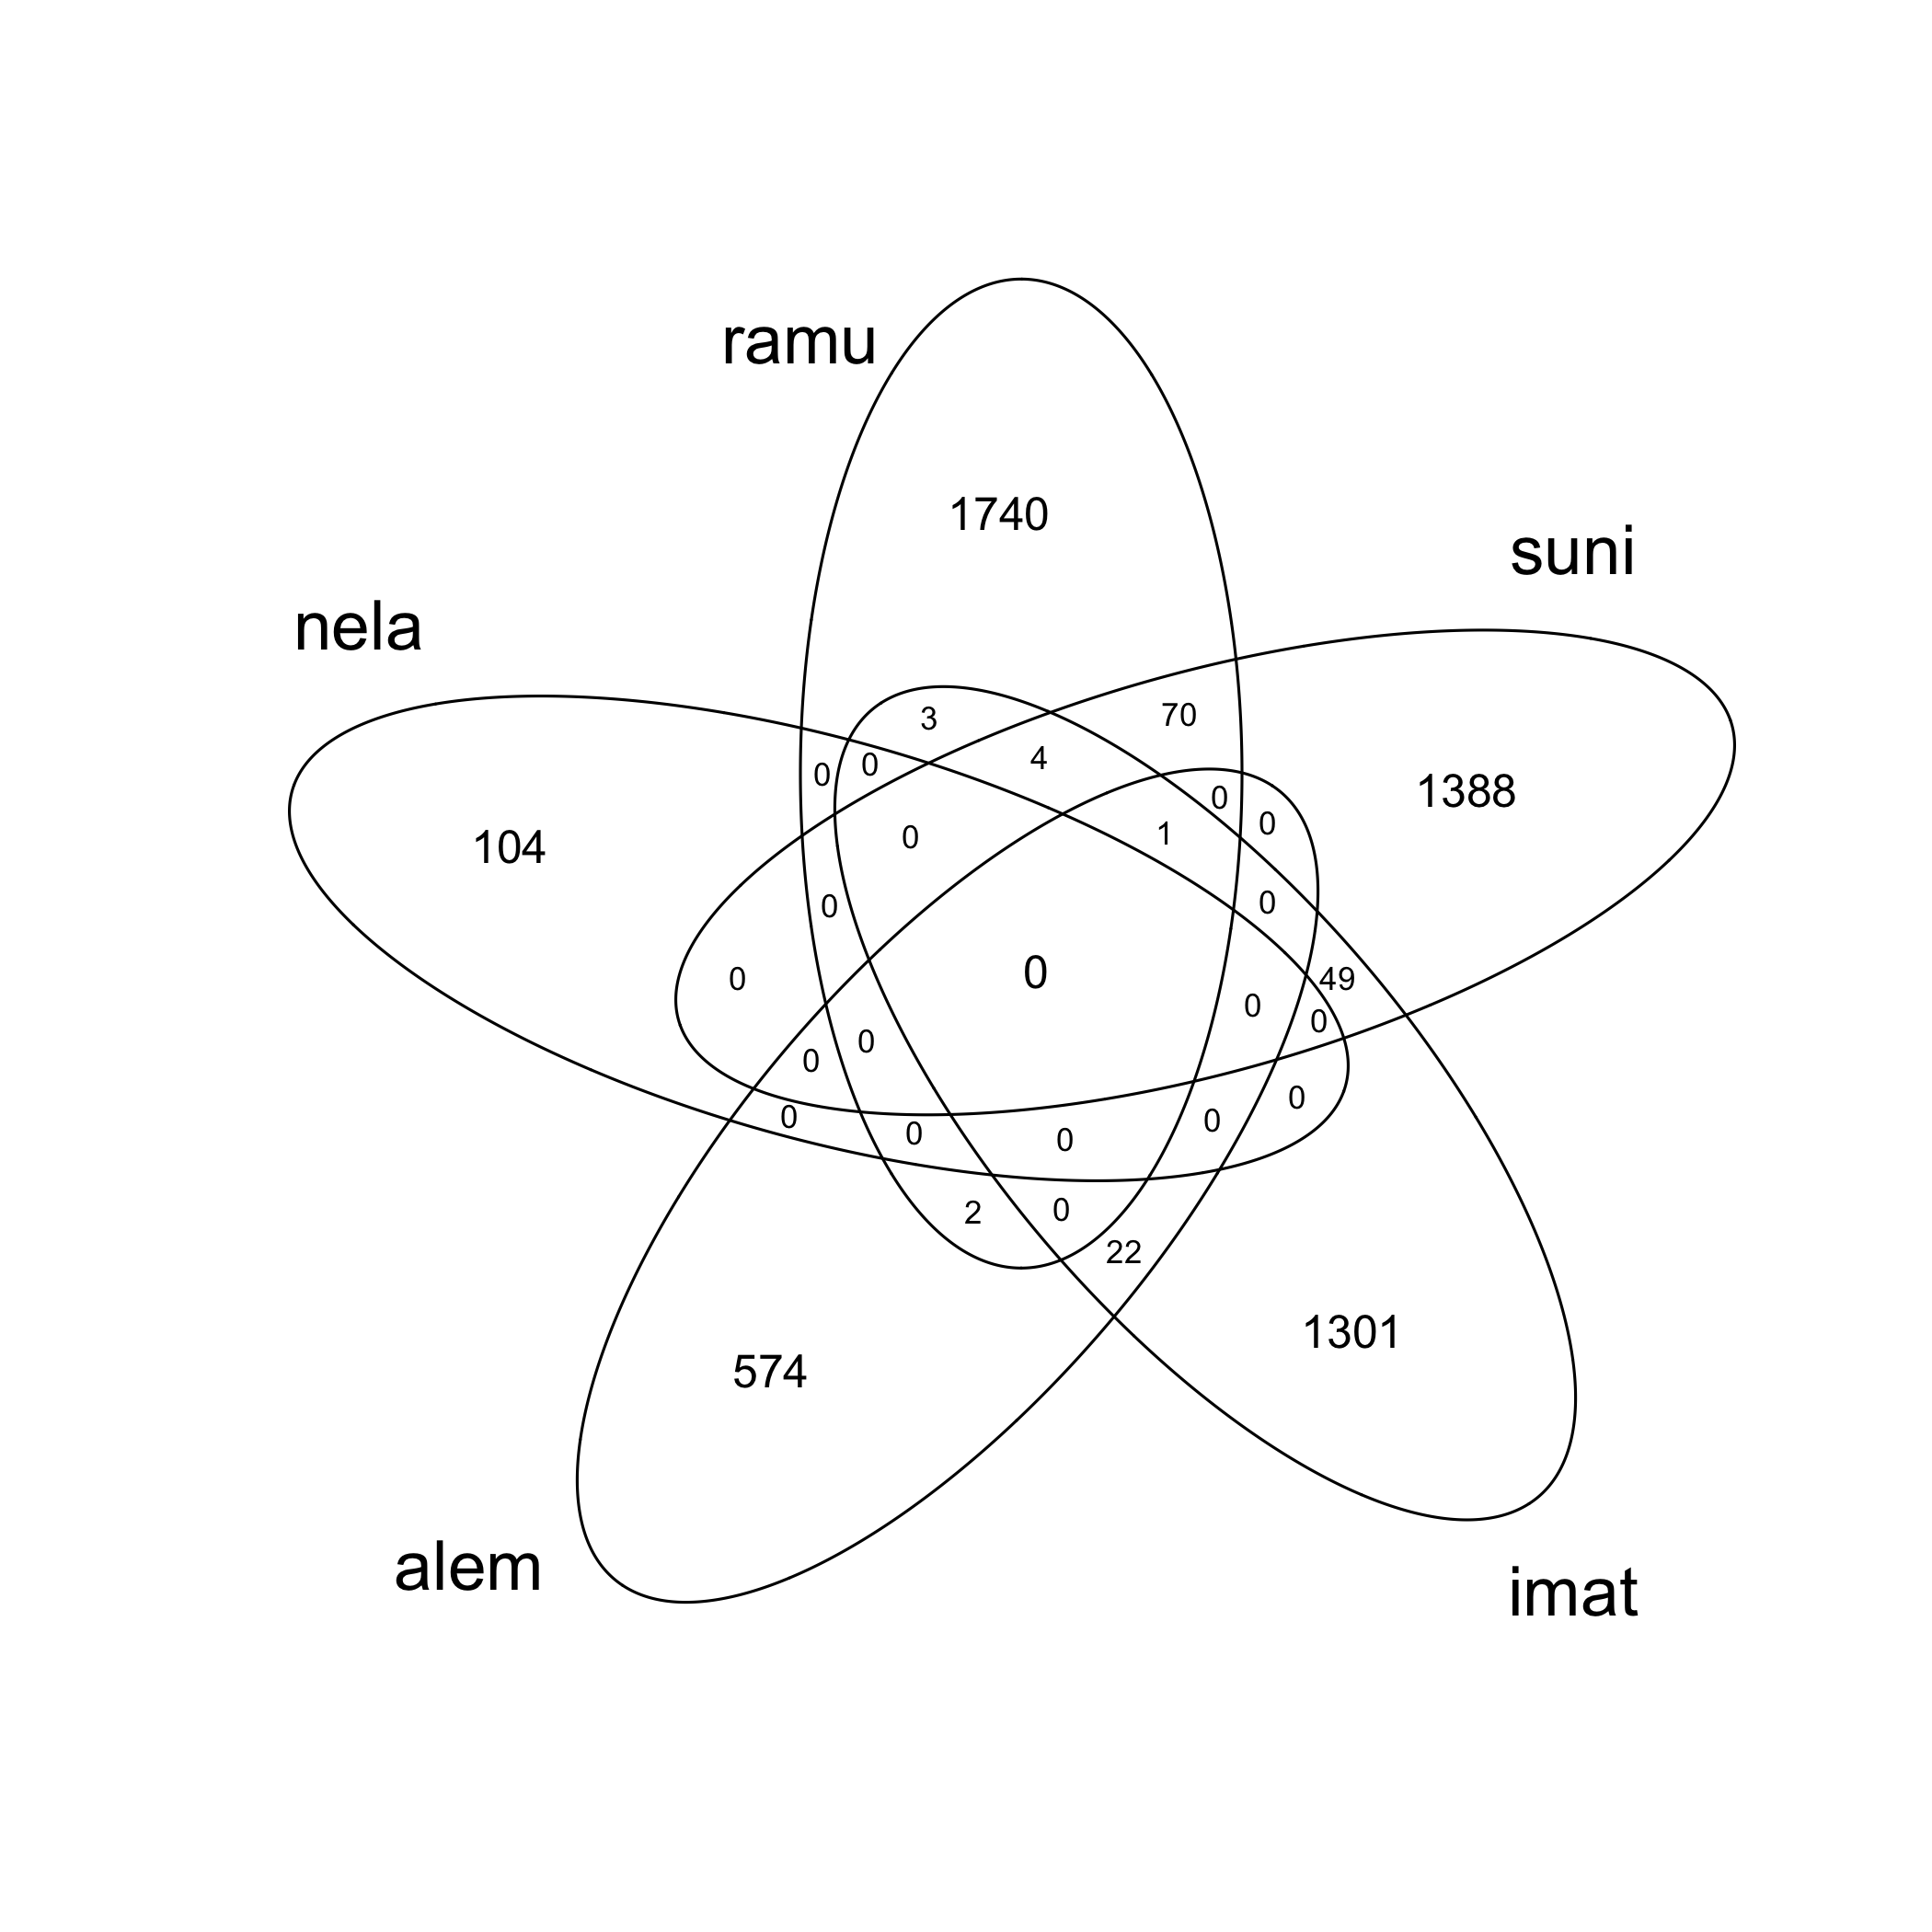
\includegraphics[scale=0.15]{citing_pmid.png}
\caption{{\bf Publications Common To First Generation References in Networks}
Intersections were calculated across all five networks for citing\_pmids (the first generation of references) as well as cited\_sids (the second generation of references) and displayed as a Venn diagram.
No publications are common to all five networks. A single publication is cited in four of five networks. Abbreviations: alem (Alemtuzumab),imat (Imatinib), nela (Nelarabine), ramu (Ramucirumab), suni(Sunitinib).}
\label{fig1}
\end{figure}

\begin{figure}[!h]
\centering
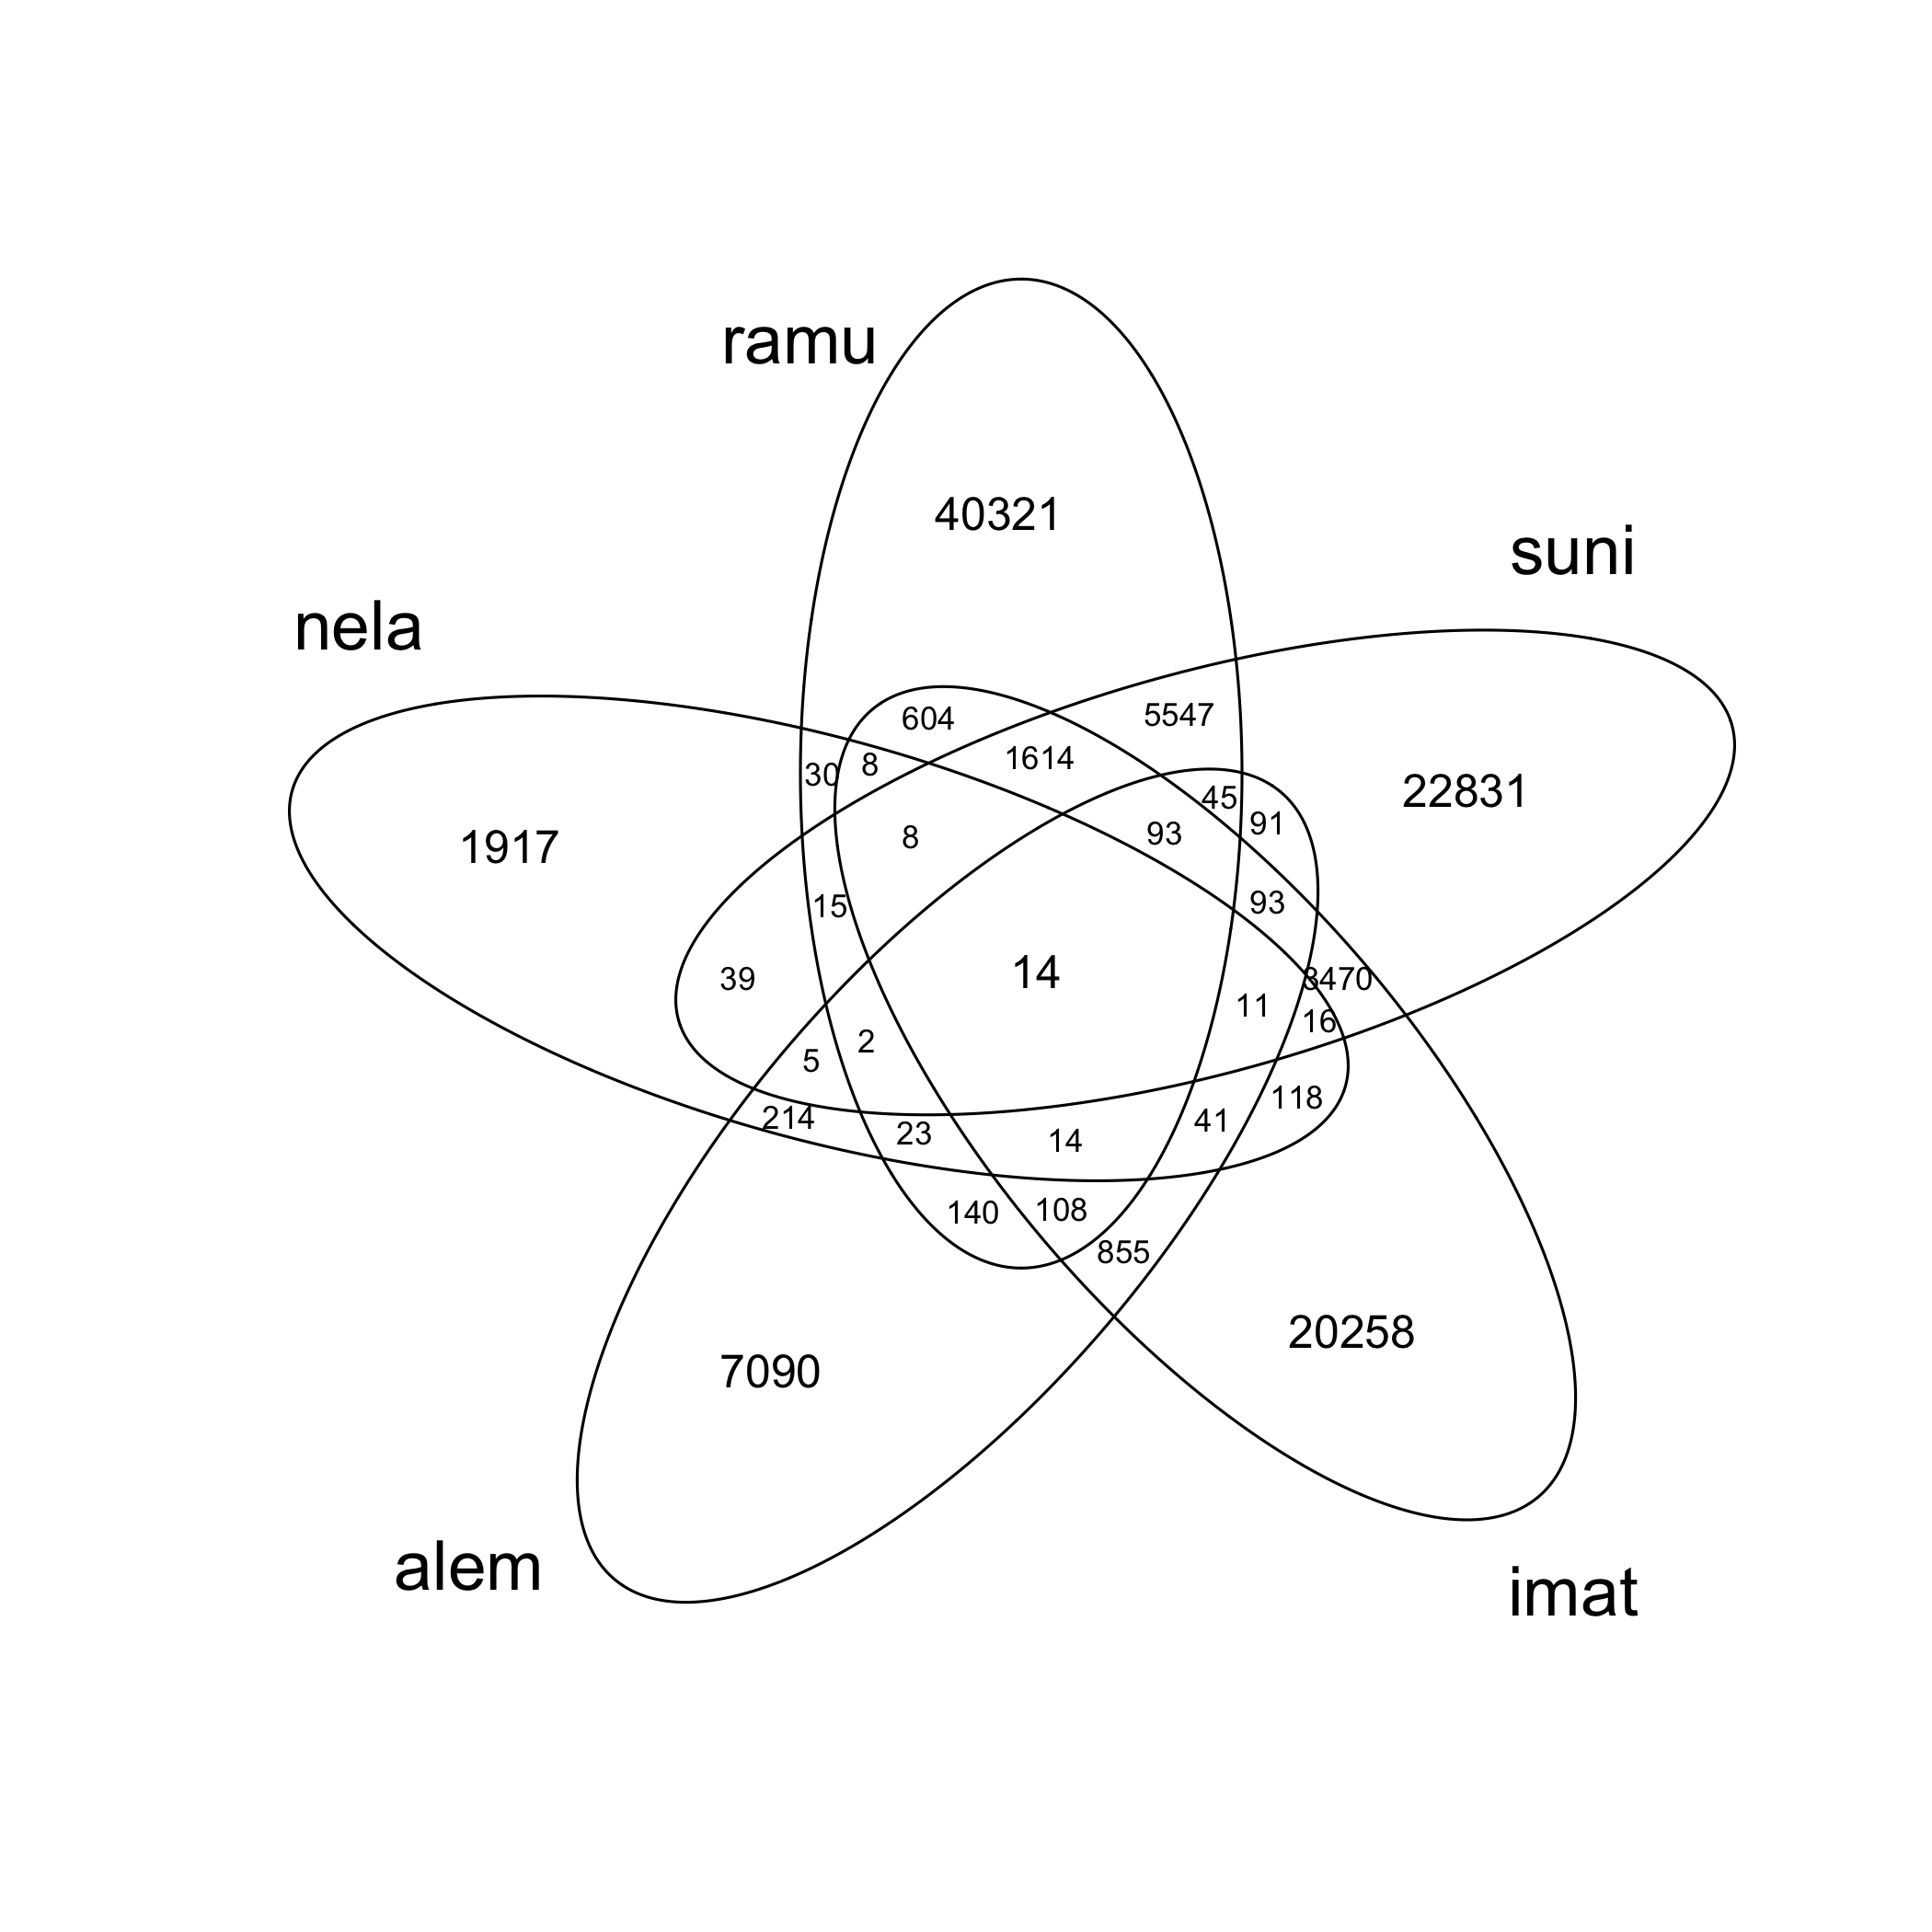
\includegraphics[scale=0.15]{cited_sid.png}
\caption{{\bf Publications Common To Second Generation References in Networks}
Intersections were calculated across all five networks for cited\_sids (the first generation of references) as well as cited\_sids (the second generation of references) and displayed as a Venn diagram.
14  publications are common to all five networks. Abbreviations: alem (Alemtuzumab), imat (Imatinib), nela (Nelarabine), ramu (Ramucirumab), suni(Sunitinib).}
\label{fig2}
\end{figure}

\subsection*{Network Features}
\subsection*{Intersection Across Networks} this is a 
\subsection*{Supporting awards and peer-review}
\subsection*{Future Directions}

\begin{table}[!ht]
%\begin{adjustwidth}{-0.51in}{0in} % Comment out/remove adjustwidth environment if table fits in text column.
\centering
\vspace{2.5 mm}
\scalebox{0.8}{
\begin{tabular}{|l| l| l| l| l| l| l| l|}
\hline
alem(A) & imat(I) & nela(N) & ramu(R) & suni(S) & combination  & intersection\_count &no\_of\_drugs\\ 
 \hline
%\multicolumn{4}{|l|}{\bf Heading1} & \multicolumn{4}{|l|}{\bf Heading2}\\ \thickhline
X & X & X & X & X & AINRS &  \textbf{14} & 5 \\ 
\hline
X & X &  & X & X & AIRS & \textbf{107} & 4 \\ 
\hline
X & X & X & X &  & AINR &  28 & 4 \\ 
\hline
X & X & X &  & X & AINS &  25 & 4 \\ 
\hline
& X & X & X & X & INRS &  22 & 4 \\ 
\hline
X &  & X & X & X & ANRS &  16 & 4 \\ 
\hline 
& X &  & X & X & IRS & \textbf{1762} & 3 \\ 
\hline
X & X &  & X &  & AIR & 231 & 3 \\ 
\hline
X & X &  &  & X & AIS & 211 & 3 \\ 
\hline
X &  &  & X & X & ARS & 156 & 3 \\ 
\hline
X & X & X &  &  & AIN &  81 & 3 \\ 
\hline
X &  & X & X &  & ANR &  56 & 3 \\ 
\hline 
& X & X &  & X & INS &  49 & 3 \\ 
\hline
& X & X & X &  & INR &  44 & 3 \\ 
\hline
 &  & X & X & X & NRS &  40 & 3 \\ 
\hline
X &  & X &  & X & ANS &  32 & 3 \\ 
\hline 
&  &  & X & X & RS & \textbf{7442} & 2 \\ 
\hline
& X &  &  & X & IS & 5415 & 2 \\ 
\hline
& X &  & X &  & IR & 2507 & 2 \\ 
\hline
X & X &  &  &  & AI & 1240 & 2 \\ 
\hline
X &  &  & X &  & AR & 448 & 2 \\ 
\hline
X &  &  &  & X & AS & 359 & 2 \\ 
\hline
X &  & X &  &  & AN & 334 & 2 \\ 
\hline 
& X & X &  &  & IN & 232 & 2 \\ 
\hline
&  & X & X &  & NR & 115 & 2 \\ 
\hline 
 &  & X &  & X & NS & 111 & 2 \\ 
\hline
&  &  & X &  & R & \textbf{49006} & 1 \\ 
\hline 
&  &  &  & X & S & 34257 & 1 \\ 
\hline 
& X &  &  &  & I & 27706 & 1 \\ 
\hline
X &  &  &  &  & A & 8978 & 1 \\ 
\hline
&  & X &  &  & N & 2498 & 1 \\ 
\hline
\end{tabular}}
\vspace{2.5 mm}
\caption{
{\bf Intersecting Publications Across Networks} Intersections were calculated for the set of publications associated with each network. Both citing and cited references were included in each set and  Scopus identifiers were used to to minimize information loss (Table 2). Intersection counts are shown for all possible combinations of the five therapeutics. The largest intersection count in each combination group is shown in boldface. Therapeutic names are abbreviated as follows: alem (Alemtuzumab), imat(Imatinib), nela (Nelarabine), ramu (Ramucirumab), suni (Sunitinib). }







%\begin{flushleft} Intersections were calculated for the set of publications associated with each network. Both citing and cited references were included in each set and  Scopus Ids were used as identifiers to minimize loss of data when mapping back to pmids. Intersection counts are shown for all possible combinations of the five therapeutics. The largest intersection count in each combination group is shown in boldface.
%\end{flushleft}
\label{table3}
%\end{adjustwidth}
\end{table}

%PLOS does not support heading levels beyond the 3rd (no 4th level headings).
\subsection*{\lorem\ and \ipsum\ Nunc blandit a tortor.}
\subsubsection*{3rd Level Heading.} 

Maecenas convallis mauris sit amet sem ultrices gravida. Etiam eget sapien nibh. Sed ac ipsum eget enim egestas ullamcorper nec euismod ligula. Curabitur fringilla pulvinar lectus consectetur pellentesque. Quisque augue sem, tincidunt sit amet feugiat eget, ullamcorper sed velit. Sed non aliquet felis. Lorem ipsum dolor sit amet, consectetur adipiscing elit. Mauris commodo justo ac dui pretium imperdiet. Sed suscipit iaculis mi at feugiat. 

\begin{enumerate}
	\item{react}
	\item{diffuse free particles}
	\item{increment time by dt and go to 1}
\end{enumerate}

\subsection*{Sed ac quam id nisi malesuada congue.}

Nulla mi mi, venenatis sed ipsum varius, volutpat euismod diam. Proin rutrum vel massa non gravida. Quisque tempor sem et dignissim rutrum. Lorem ipsum dolor sit amet, consectetur adipiscing elit. Morbi at justo vitae nulla elementum commodo eu id massa. In vitae diam ac augue semper tincidunt eu ut eros. Fusce fringilla erat porttitor lectus cursus, vel sagittis arcu lobortis. Aliquam in enim semper, aliquam massa id, cursus neque. Praesent faucibus semper libero.

\begin{itemize}
	\item First bulleted item.
	\item Second bulleted item.
	\item Third bulleted item.
\end{itemize}

%\section*{Discussion}


\section*{Conclusion}

CO\textsubscript{2} Maecenas convallis mauris sit amet sem ultrices gravida. Etiam eget sapien nibh. Sed ac ipsum eget enim egestas ullamcorper nec euismod ligula. Curabitur fringilla pulvinar lectus consectetur pellentesque. Quisque augue sem, tincidunt sit amet feugiat eget, ullamcorper sed velit. 

Sed non aliquet felis. Lorem ipsum dolor sit amet, consectetur adipiscing elit. Mauris commodo justo ac dui pretium imperdiet. Sed suscipit iaculis mi at feugiat. Ut neque ipsum, luctus id lacus ut, laoreet scelerisque urna. Phasellus venenatis, tortor nec vestibulum mattis, massa tortor interdum felis, nec pellentesque metus tortor nec nisl. Ut ornare mauris tellus, vel dapibus arcu suscipit sed. Nam condimentum sem eget mollis euismod. Nullam dui urna, gravida venenatis dui et, tincidunt sodales ex. Nunc est dui, sodales sed mauris nec, auctor sagittis leo. Aliquam tincidunt, ex in facilisis elementum, libero lectus luctus est, non vulputate nisl augue at dolor. For more information, see \nameref{S1_Appendix}.

\section*{Supporting Information}

% Include only the SI item label in the paragraph heading. Use the \nameref{label} command to cite SI items in the text.
\paragraph*{S1 Fig.}
\label{S1_Fig}
{\bf Bold the title sentence.} Add descriptive text after the title of the item (optional).

\paragraph*{S2 Fig.}
\label{S2_Fig}
{\bf Lorem Ipsum.} Maecenas convallis mauris sit amet sem ultrices gravida. Etiam eget sapien nibh. Sed ac ipsum eget enim egestas ullamcorper nec euismod ligula. Curabitur fringilla pulvinar lectus consectetur pellentesque.

\paragraph*{S1 File.}
\label{S1_File}
{\bf Lorem Ipsum.}  Maecenas convallis mauris sit amet sem ultrices gravida. Etiam eget sapien nibh. Sed ac ipsum eget enim egestas ullamcorper nec euismod ligula. Curabitur fringilla pulvinar lectus consectetur pellentesque.

\paragraph*{S1 Video.}
\label{S1_Video}
{\bf Lorem Ipsum.}  Maecenas convallis mauris sit amet sem ultrices gravida. Etiam eget sapien nibh. Sed ac ipsum eget enim egestas ullamcorper nec euismod ligula. Curabitur fringilla pulvinar lectus consectetur pellentesque.

\paragraph*{S1 Appendix.}
\label{S1_Appendix}
{\bf Lorem Ipsum.} Maecenas convallis mauris sit amet sem ultrices gravida. Etiam eget sapien nibh. Sed ac ipsum eget enim egestas ullamcorper nec euismod ligula. Curabitur fringilla pulvinar lectus consectetur pellentesque.

\paragraph*{S1 Table.}
\label{S1_Table}
{\bf Lorem Ipsum.} Maecenas convallis mauris sit amet sem ultrices gravida. Etiam eget sapien nibh. Sed ac ipsum eget enim egestas ullamcorper nec euismod ligula. Curabitur fringilla pulvinar lectus consectetur pellentesque.

\section*{Acknowledgments}
Cras egestas velit mauris, eu mollis turpis pellentesque sit amet. Interdum et malesuada fames ac ante ipsum primis in faucibus. Nam id pretium nisi. Sed ac quam id nisi malesuada congue. Sed interdum aliquet augue, at pellentesque quam rhoncus vitae.

\begin{eqnarray}
\label{eq:schemeP} 
	\mathrm{P_Y} = \underbrace{H(Y_n) - H(Y_n|\mathbf{V}^{Y}_{n})}_{S_Y} + \underbrace{H(Y_n|\mathbf{V}^{Y}_{n})- H(Y_n|\mathbf{V}^{X,Y}_{n})}_{T_{X\rightarrow Y}},
\end{eqnarray}

\nolinenumbers

\begin{figure}[!h]
\caption{{\bf Bold the figure title.}
Figure caption text here, please use this space for the figure panel descriptions instead of using subfigure commands. A: Lorem ipsum dolor sit amet. B: Consectetur adipiscing elit.}
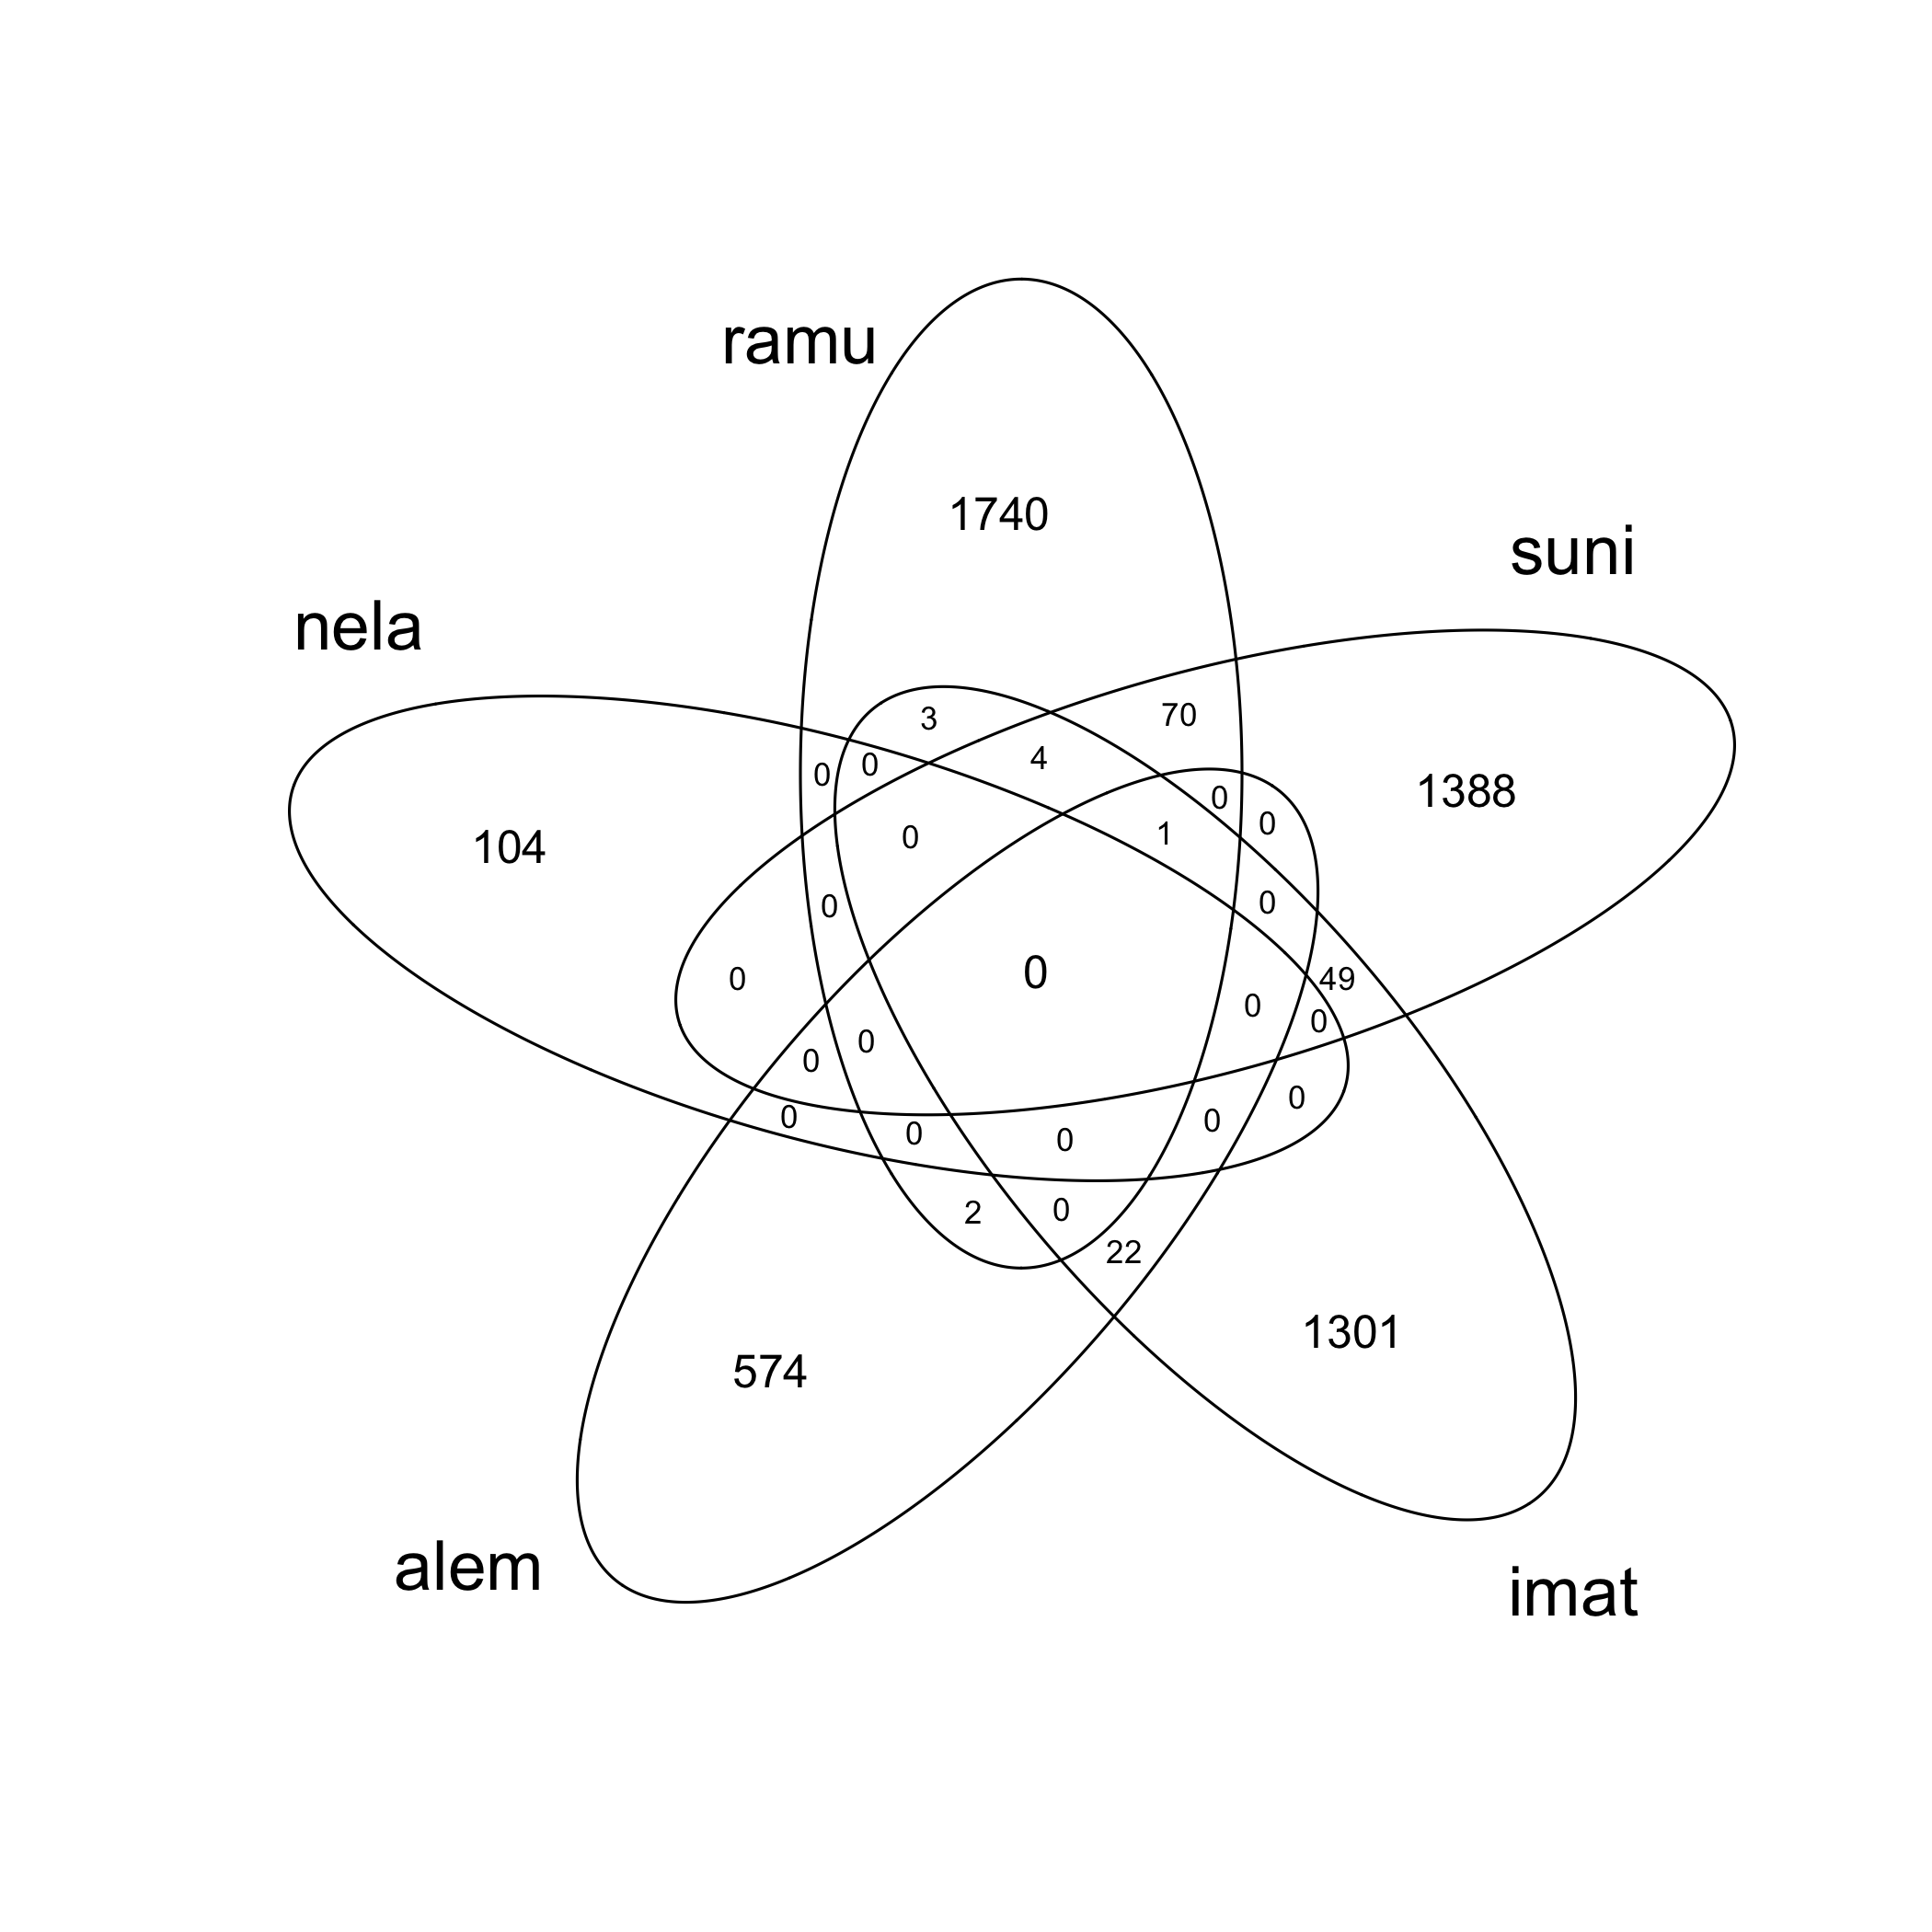
\includegraphics{citing_pmid.png}
\label{fig2}
\end{figure}

% Either type in your references using
% \begin{thebibliography}{}
% \bibitem{}
% Text
% \end{thebibliography}
%
% or
%
% Compile your BiBTeX database using our plos2015.bst
% style file and paste the contents of your .bbl file
% here.
% 
\begin{thebibliography}{10}

\bibitem{bibWilliams}
Williams RS, Lotia S., Holloway AK, Pico AR.
\newblock {{F}rom Scientific Discovery to Cures: Bright Stars within a Galaxy.}
\newblock Cell. 2015 Sep; 163:21--23

\bibitem{bibLauer}
Lauer MS.
\newblock {{P}CSK9 Inhibitors: Lots of Work Done, Lots More to Do.}
\newblock Ann Intern Med. 2016 Mar; 164(9):624-625.

\bibitem{bibChan}
O'Shea JJ, Kanno, Y., Chan AC.
\newblock {{I}n Search of Magic Bullets: The Golden Age of Immunotherapeutics}
\newblock Cell. 2014 Mar; 157:227-240

\bibitem{bibMaldame}
Maldame, J.
\newblock {{T}he Importance Of The History Of Science In Intellectual Formation}
\newblock Scripta Varia 2002 104:237-248

\bibitem{bibFDA}
Federal Drug Administration.
\newblock {{D}rugs@FDA: FDA Approved Drug Products}
\newblock https://www.accessdata.fda.gov/scripts/cder/daf/

\bibitem{bibNIHExPORTER}
National Institutes of Health.
\newblock {{N}IH ExPORTER}
\newblock https://exporter.nih.gov/

\bibitem{bibGooglePatents}
Google Corporation
\newblock {{G}oogle Patents}
\newblock https://patents.google.com/

\bibitem{bibKohler}
K\"ohler, G., Milstein, C.
\newblock { {C}ontinuous cultures of fused cells secreting antibody of predefined specificity.}
\newblock Nature. 1975 256: 495?497
 
\bibitem{bibn}
Magwire MM, Bayer F, Webster CL, Cao C, Jiggins FM.
\newblock {{S}uccessive increases in the resistance of {D}rosophila to viral
infection through a transposon insertion followed by a {D}uplication}.
\newblock PLoS Genet. 2011 Oct;7(10):e1002337.

\end{thebibliography}

\end{document}

